\documentclass[preprint,12pt]{elsarticle} % http://www.latextemplates.com/template/elseviers-elsarticle-document-class
\usepackage{lipsum} % To add some random latin text


%%%% THE ELSEVIER DOCOMENT CLASS LET US PUT THE NAME OF A JOURNAL
\journal{Super Journal of Good Stuff}



\begin{document}

%%%% IT ALSO FORMATS ALL THE FRONT MATTER STUFF LIKE TITLE, AUTHOR(S), ETC.
\begin{frontmatter}
  \title{My Article Title}
  \author{My Name}
  \address{Universit\'e Laval}

  \begin{abstract}
    %% Text of abstract
    \lipsum[2]
  \end{abstract}

  \begin{keyword}
  Banana, Apple, Sand Paper
  \end{keyword}
\end{frontmatter}



%%%% THE MAIN TEXT STARTS HERE...
\section{Introduction}



%%%% ADD SOME CITATIONS (THE FIRST = IN-TEXT. THE SECOND = INDIRECT)
\citet{huntington1993clash} says a lot of things. Things are not always what we want them to be \citep{skocpol1999bringing}.





%%%% ADD RANDOM LATIN TEXT
\lipsum[1]





%%%% ADD OUR TWO FIGURES
\begin{figure}[h!]
  \caption{My Super Histogram}
  \centering
  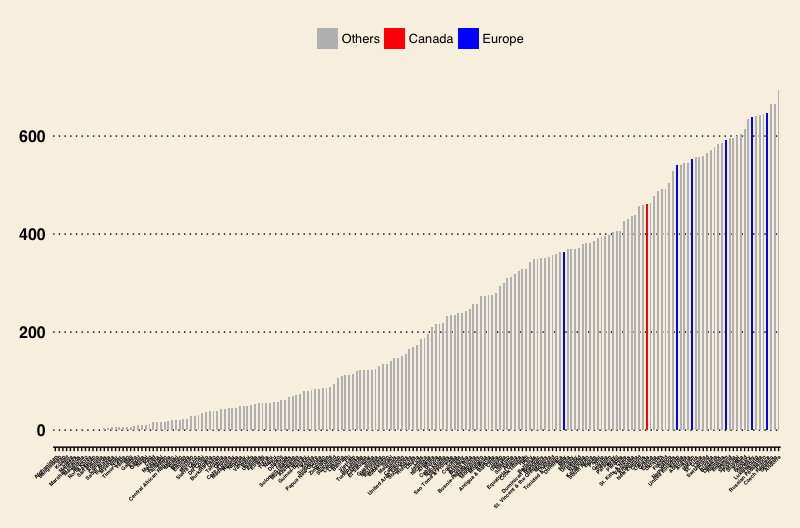
\includegraphics[width=1\textwidth]{AlcoholConsumptionHistogram}
\end{figure}

\begin{figure}[h!]
  \caption{My Super Map}
  \centering
  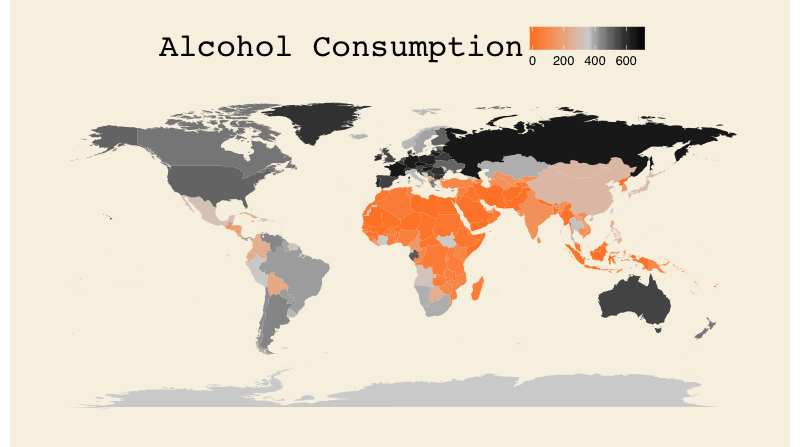
\includegraphics[width=1\textwidth]{AlcoholConsumptionMap}
\end{figure}





%%%% ADD RANDOM LATIN TEXT
\lipsum[2]





%%%% ADD A REGRESSION TABLE





%%%% PRINT THE BIBLIOGRAPHY
\bibliographystyle{model5-names}
\biboptions{authoryear}
\bibliography{MyBibliography}



\end{document}

%%
%% End of file `elsarticle-template-1-num.tex'.
